\chapter{Experimental Results} \label{ch:Exp_Results}

\section{Long Walk Trials}

Figures~\ref{fig:longWalk1_xyz}--\ref{fig:longWalk5_xyz} plot the vehicle's $x$-, $y$-, and $z$-coordinates over time. These plots demonstrate that the UKF's pose estimates were able to track the vehicle's $y$-position accurately over the length of each long walk trial. The plots also show that the UKF pose estimates exhibit aberrant behavior causing the vehicle's $z$-position to rise more and more the farther the vehicle moves from the origin. The shaded region in Figure~\ref{fig:longWalk1_xyz} clearly highlights this behavior. The vehicle's estimated altitude rises steadily to a maximum of about 1.4~meters, although in truth the vehicle's altitude was constant throughout. The vehicle's maximum vertical error coincides with its maximal displacement from $\left( 0,\ 0,\ 0 \right)$.

In each trial, the UKF output showed increased ``shakiness'' in the form of large oscillations as the vehicle's $y$-position increased. As the mobile test stand moved farther and farther away from the origin, visualizations of the output showed erroneous vertical spikes in conjunction with the altitude generally trending upward. The magnitude of these spikes increased with displacement from the origin, always achieving a maximal magnitude at the point of maximal displacement. Moreover, this behavior was coupled with aberrant displacements along the $x$-axis as well. This behavior seems to follow the supposition posited earlier in Chapter~\ref{ch:Exp_Design} that the ROS PTAM implementation was not correctly eliminating lens distortion and, as a result, was perceiving a bowl-shaped world. If PTAM's view of the environment were curved, the large erroneous readings in $x$ and $z$ would reasonably be coupled to displacement along the $y$-axis, as the $y$-displacement would affect the vehicle's ``height'' along the inside of the ``bowl.'' The farther the vehicle moved from the bottom of the bowl at the origin, the more $z$ would increase and the more $x$ would become susceptible to overestimating small lateral perturbations. This trend can be seen, to varying degrees, in all five trials, with maximal error in the $z$ coordinate being accompanied by maximal ``shakiness'' in the $x$ coordinate---all coinciding with maximal displacement from the origin.

\begin{figure}[H]
  \centering
    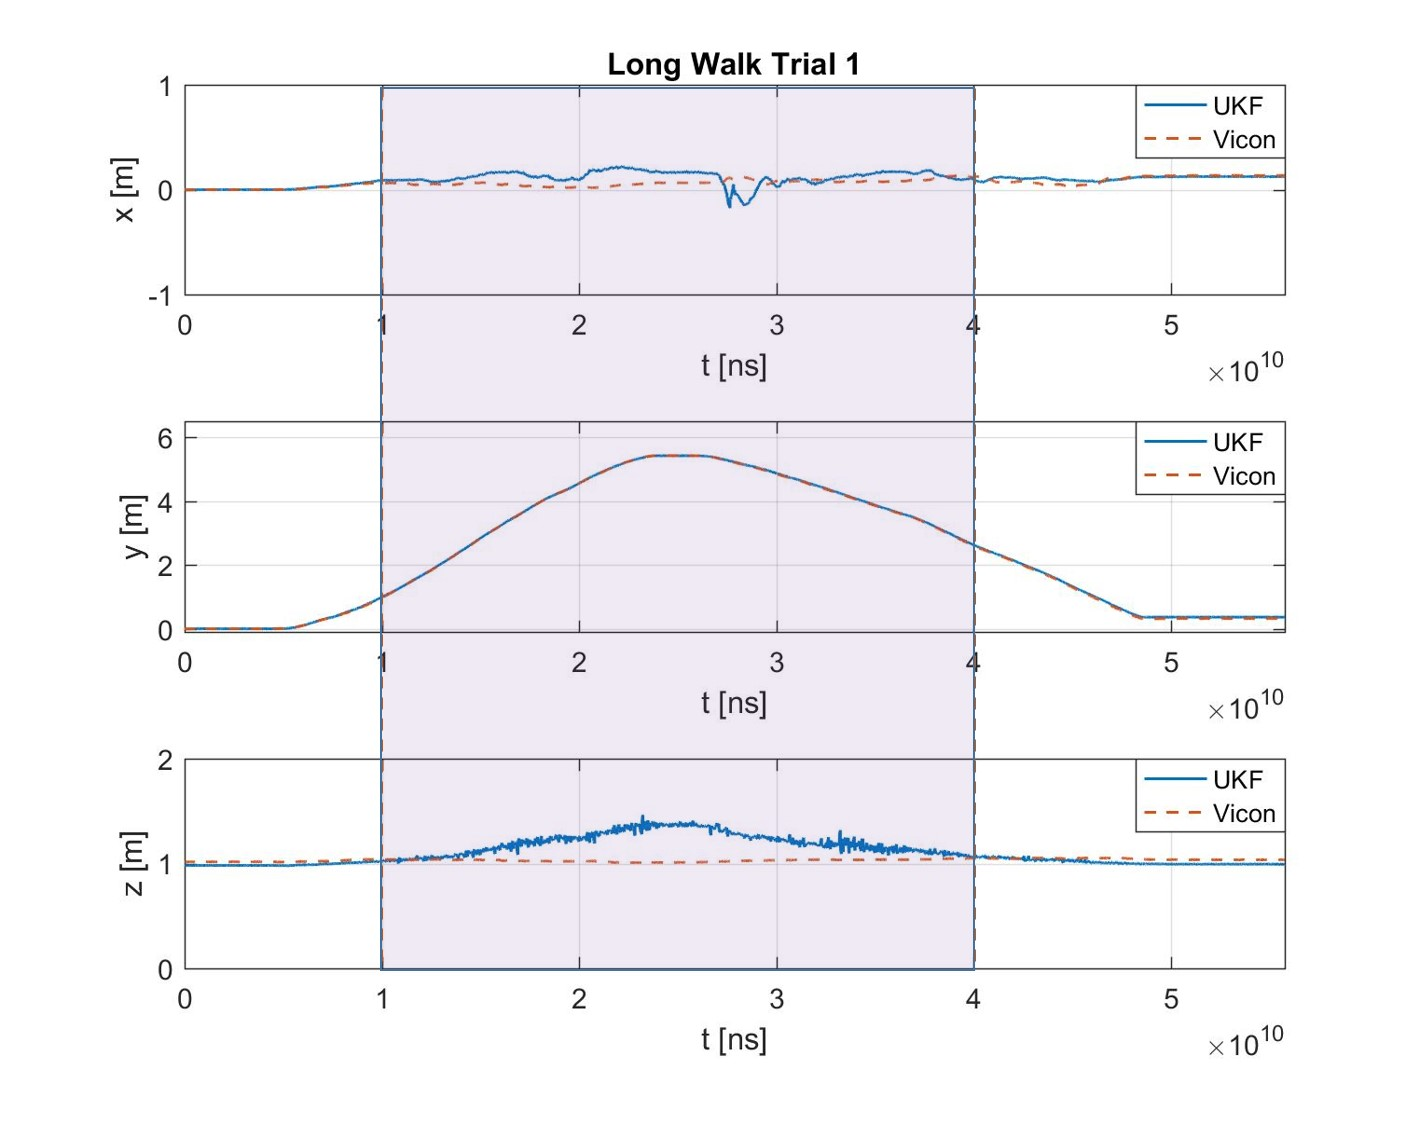
\includegraphics[width=\textwidth]{longWalk1_xyz}
  \caption[Long Walk Trial 1]{Long Walk Trial 1 coordinate plots. The shaded region highlights aberrant behavior coinciding with maximal displacement from the origin.}
  \label{fig:longWalk1_xyz}
\end{figure}

\begin{figure}[H]
  \centering
    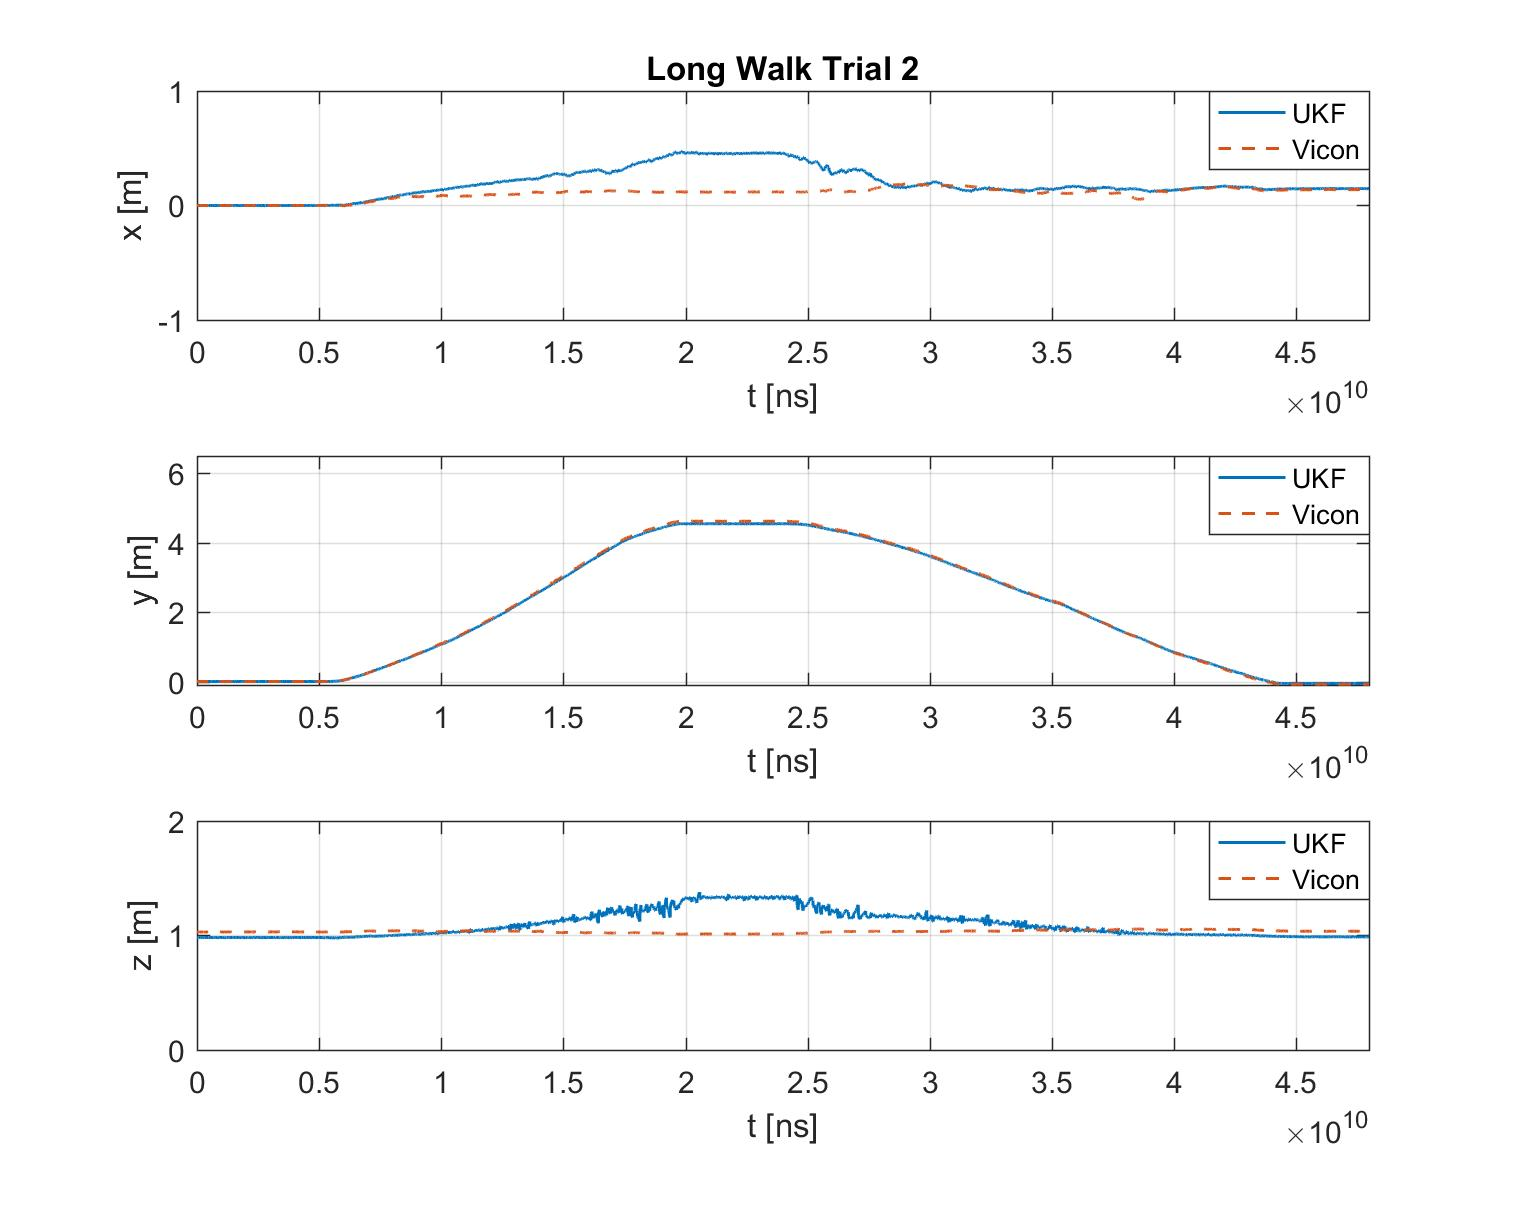
\includegraphics[width=\textwidth]{longWalk2_xyz}
  \caption[Long Walk Trial 2]{Long Walk Trial 2 coordinate plots.}
  \label{fig:longWalk2_xyz}
\end{figure}

\begin{figure}[H]
  \centering
    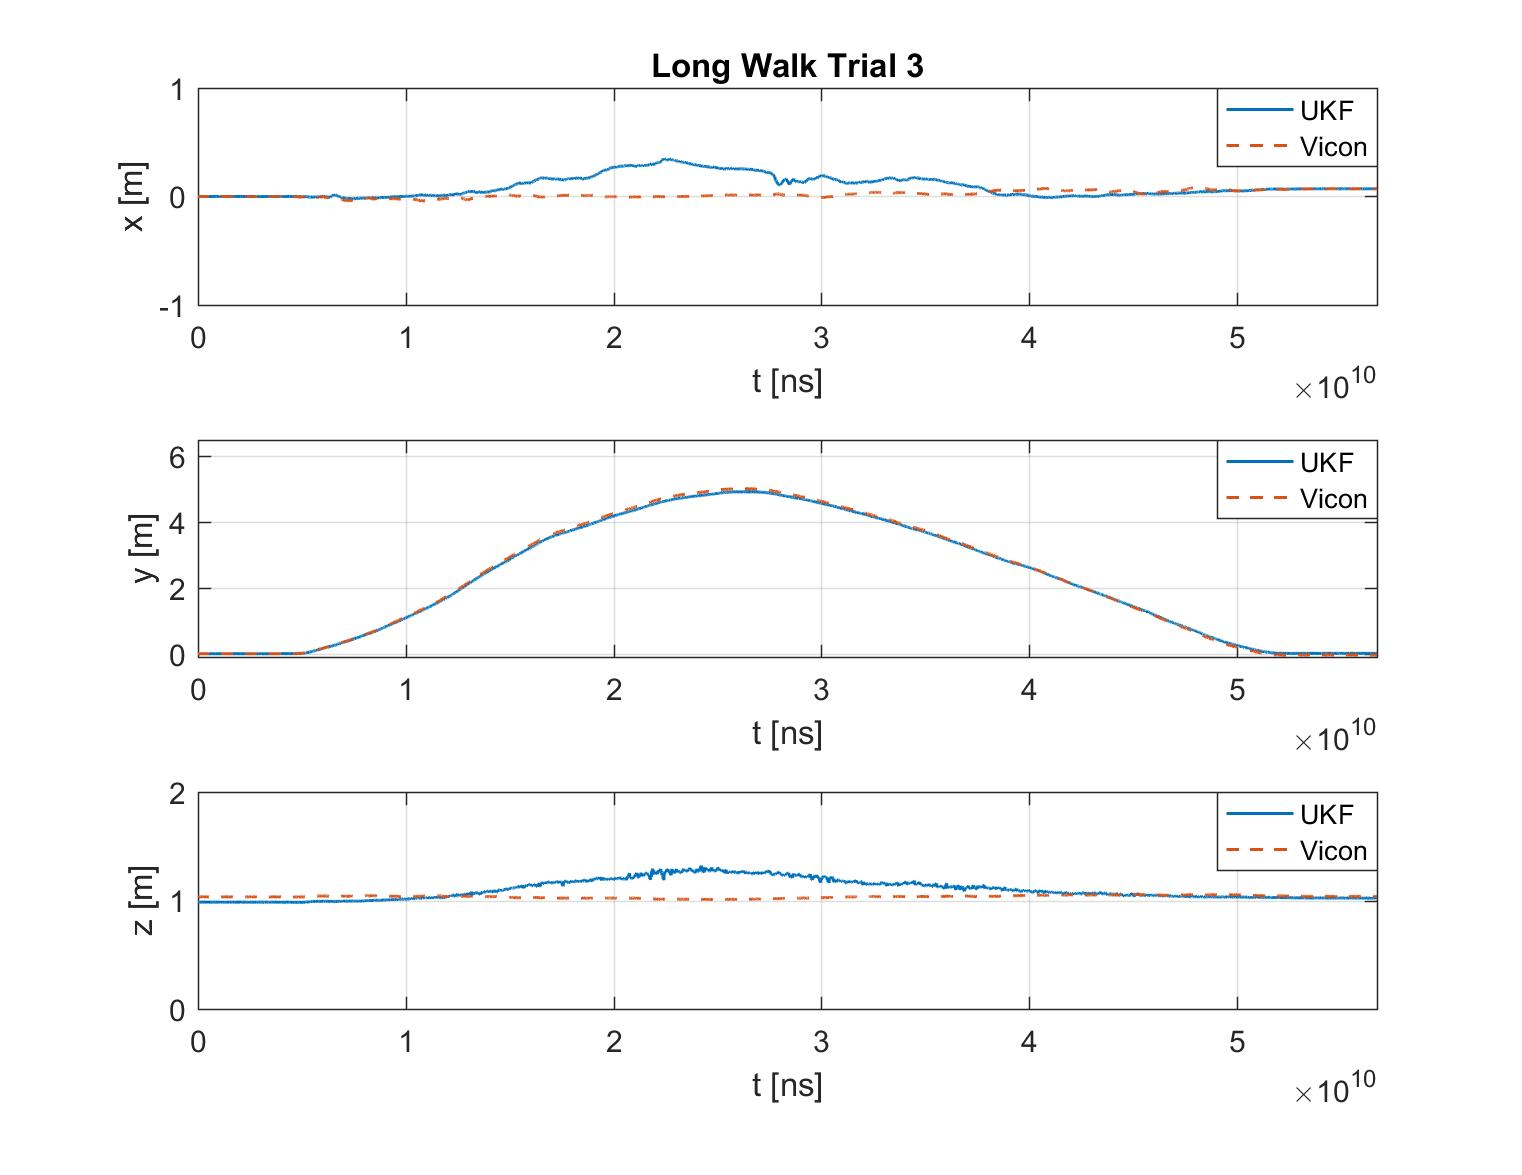
\includegraphics[width=\textwidth]{longWalk3_xyz}
  \caption[Long Walk Trial 3]{Long Walk Trial 3 coordinate plots.}
  \label{fig:longWalk3_xyz}
\end{figure}

\begin{figure}[H]
  \centering
    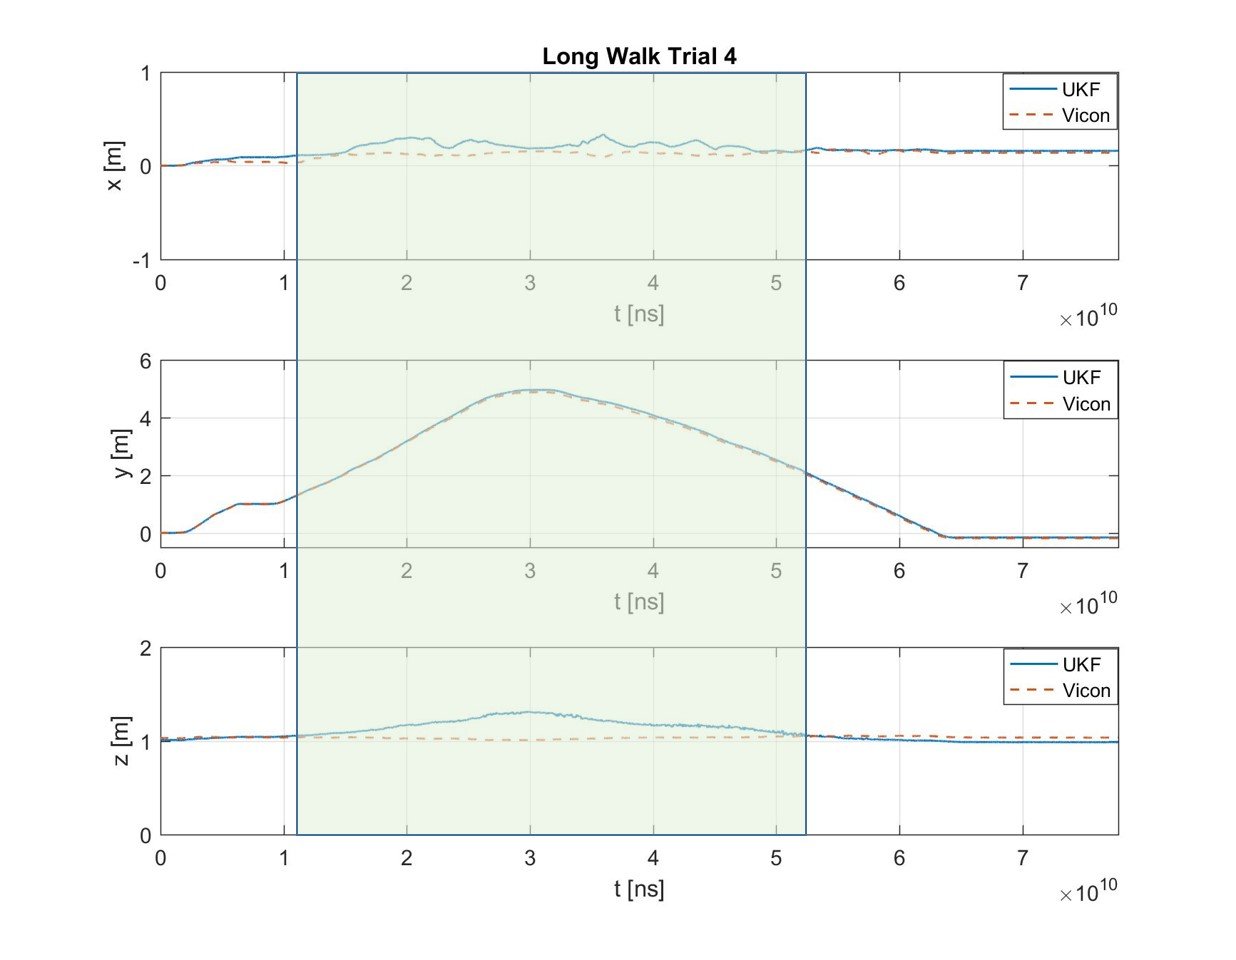
\includegraphics[width=\textwidth]{longWalk4_xyz}
  \caption[Long Walk Trial 4]{Long Walk Trial 4 coordinate plots.}
  \label{fig:longWalk4_xyz}
\end{figure}

\begin{figure}[H]
  \centering
    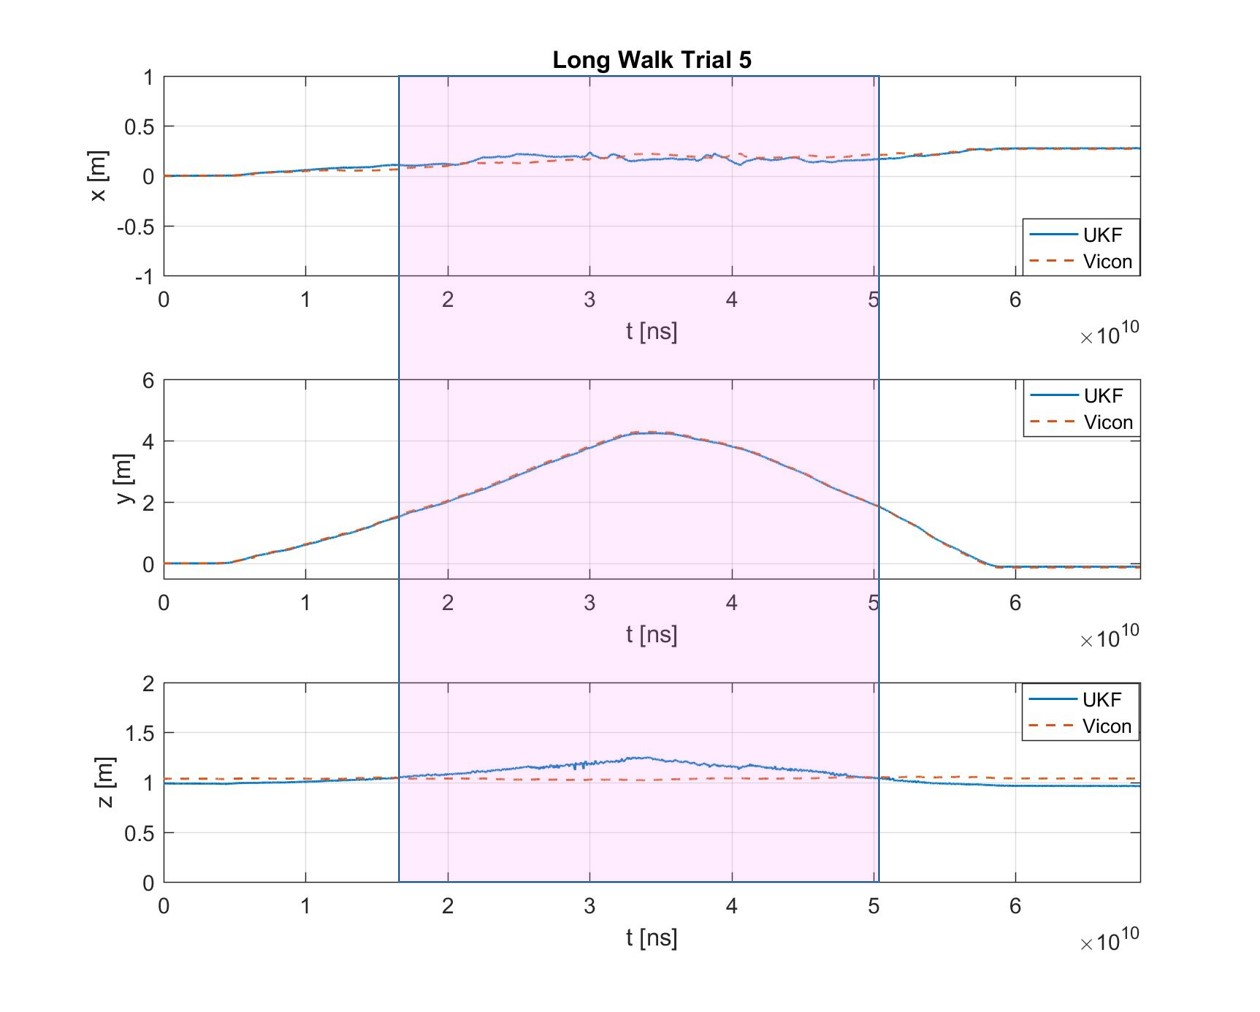
\includegraphics[width=\textwidth]{longWalk5_xyz}
  \caption[Long Walk Trial 5]{Long Walk Trial 5 coordinate plots.}
  \label{fig:longWalk5_xyz}
\end{figure}
\clearpage

\section{Box Pattern Trials}

Figures~\ref{fig:box1_3d}, \ref{fig:box2_3d}, \ref{fig:box3_3d}, \ref{fig:box4_3d}, and \ref{fig:box5_3d} plot the estimated and measured 3D trajectories of the mobile test stand during the five box pattern trials. Each of these plots exhibits the same bowl-shaped distortion seen previously in the long walk experiment. The $z$-position of the vehicle can be seen trending upward more and more the farther the vehicle moves from the origin. This causes the apparent slantedness of the estimated trajectories. This altitudinal error is most pronounced at the forward-left corner in each 3D plot, where the vehicle is farthest from the origin. The estimated trajectory also becomes noticeably shakier, in terms of vertical oscillations, in the neighborhood of the forward-left corner. These oscillations begin to appear on the first (right-side) leg of the trajectory and increase in magnitude up to the forward-left corner, at which point they begin to decrease in magnitude on the way back to the starting position.

The 2D trajectory plots (Figures~\ref{fig:box1_2d}, \ref{fig:box2_2d}, \ref{fig:box3_2d}, \ref{fig:box4_2d}, and \ref{fig:box5_2d}) are presented alongside the 3D plots to demonstrate the general accuracy of the UKF's estimates in planar motion. The UKF output follows the Vicon output faithfully, with some exceptions near the corners of the box pattern. This is caused partly by the bowl-shaped distortion mentioned previously, and partly by the fact that the mobile test stand moves on caster wheels. When the test stand changes direction, the caster wheels rotate underneath the cart, causing some lateral disturbance in the test stand's trajectory. This is particularly apparent in Figures~\ref{fig:box2_2d} and \ref{fig:box4_2d}, where a clear ``wiggling'' can be seen as the vehicle was pulled back from the top left corner of the pattern, and in Figure~\ref{fig:box5_2d}, where the estimated trajectory ``sags'' in the bottom left corner. These lateral disturbances, though small in magnitude (likely on the order of 3--5~cm) were picked up by PTAM and overestimated due to lens distortion.

Trial~3 (Figures~\ref{fig:box3_2d} and \ref{fig:box3_3d}) exhibits an anomalous $x$-directional offset along the first leg of the trajectory. This was most likely caused by inadvertent jostling of the test stand before initializing PTAM. The test stand was rotated at an angle to Vicon's $x$-axis at the outset of the trial, causing the estimated trajectory to be computed at an angle to the ground truth trajectory. Once the test stand reached the first corner, it must have been rotated slightly, causing the estimated trajectory to rejoin the ground truth measurements provided by Vicon.

\clearpage

% Box 1
\begin{figure}[p]
  \centering
    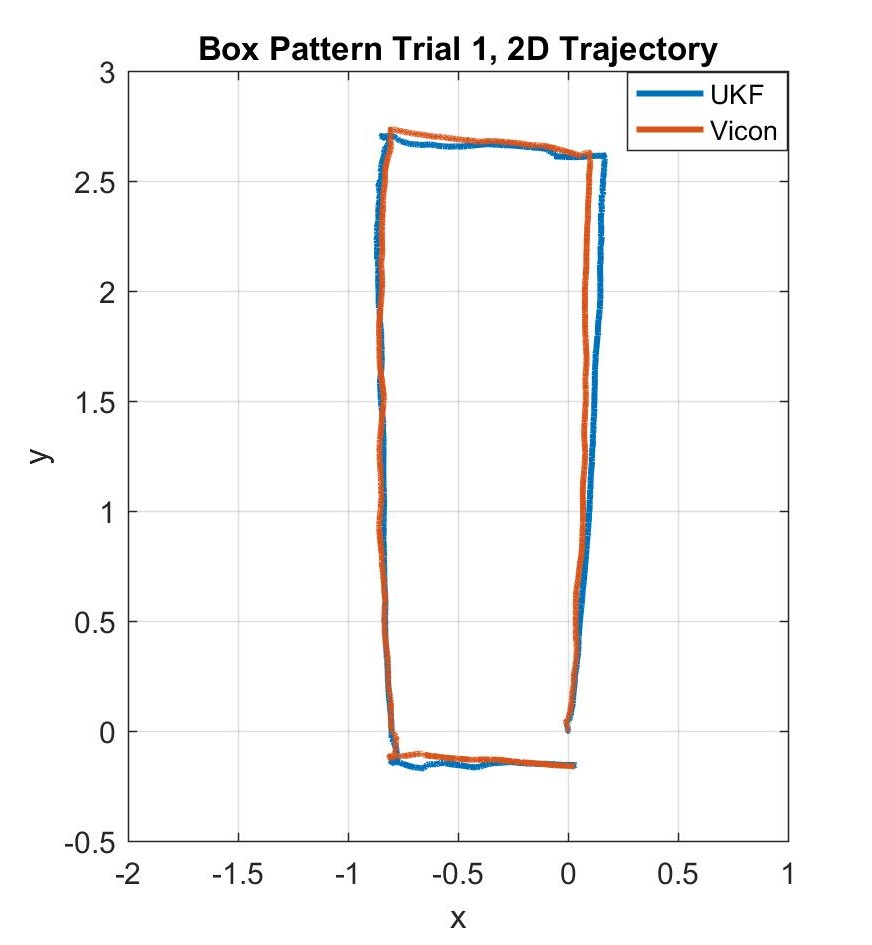
\includegraphics[height=0.6\textwidth]{box1_2d}
  \caption[Box Pattern Trial 1 2D Trajectory]{Box Pattern Trial 1 2D Trajectory.}
  \label{fig:box1_2d}
\end{figure}
\begin{figure}[p]
  \centering
    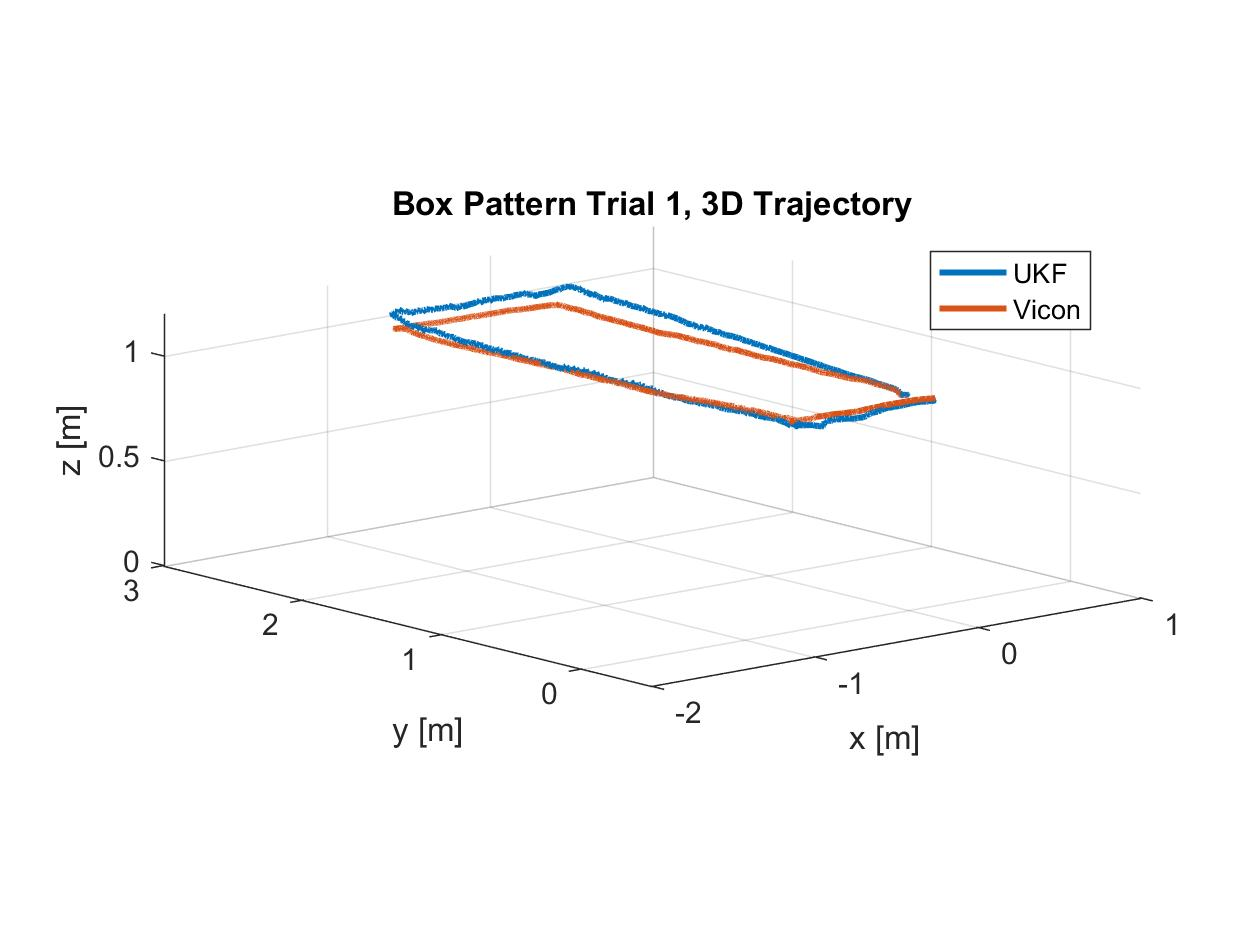
\includegraphics[height=0.7\textwidth]{box1_3d}
  \caption[Box Pattern Trial 1 3D Trajectory]{Box Pattern Trial 1 3D Trajectory.}
  \label{fig:box1_3d}
\end{figure}
\clearpage

% Box 2
\begin{figure}[p]
  \centering
    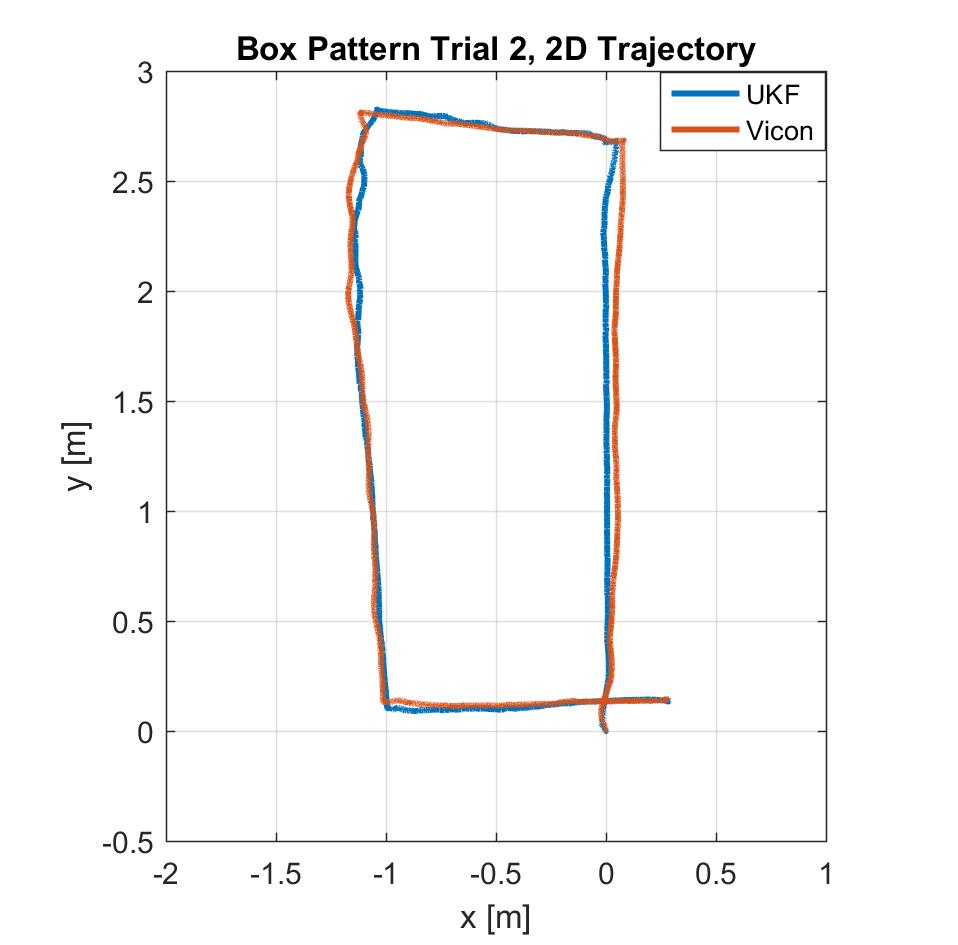
\includegraphics[height=0.6\textwidth]{box2_2d}
  \caption[Box Pattern Trial 2 2D Trajectory]{Box Pattern Trial 2 2D Trajectory.}
  \label{fig:box2_2d}
\end{figure}
\begin{figure}[p]
  \centering
    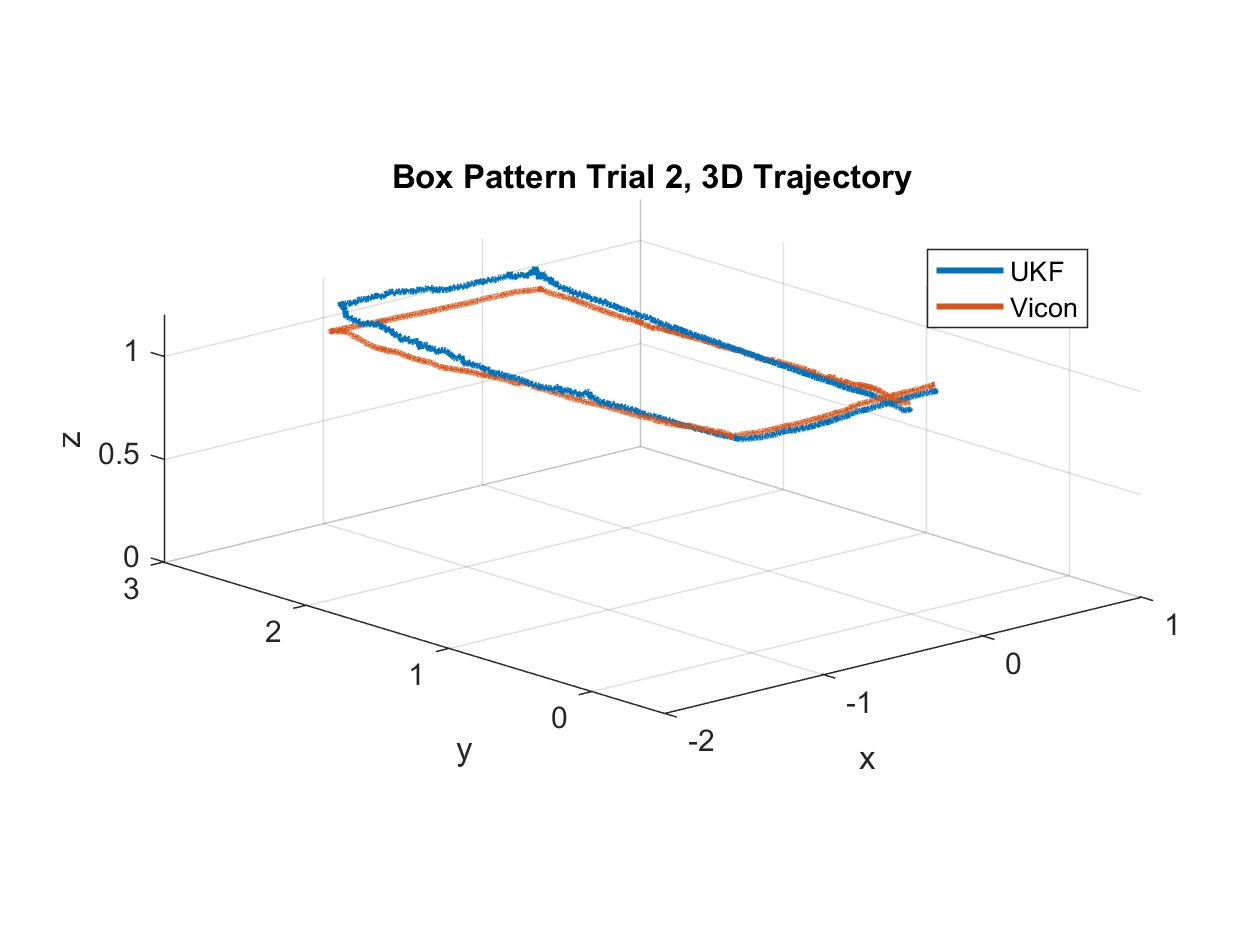
\includegraphics[height=0.7\textwidth]{box2_3d}
  \caption[Box Pattern Trial 2 3D Trajectory]{Box Pattern Trial 2 3D Trajectory.}
  \label{fig:box2_3d}
\end{figure}
\clearpage

% Box 3
\begin{figure}[p]
  \centering
    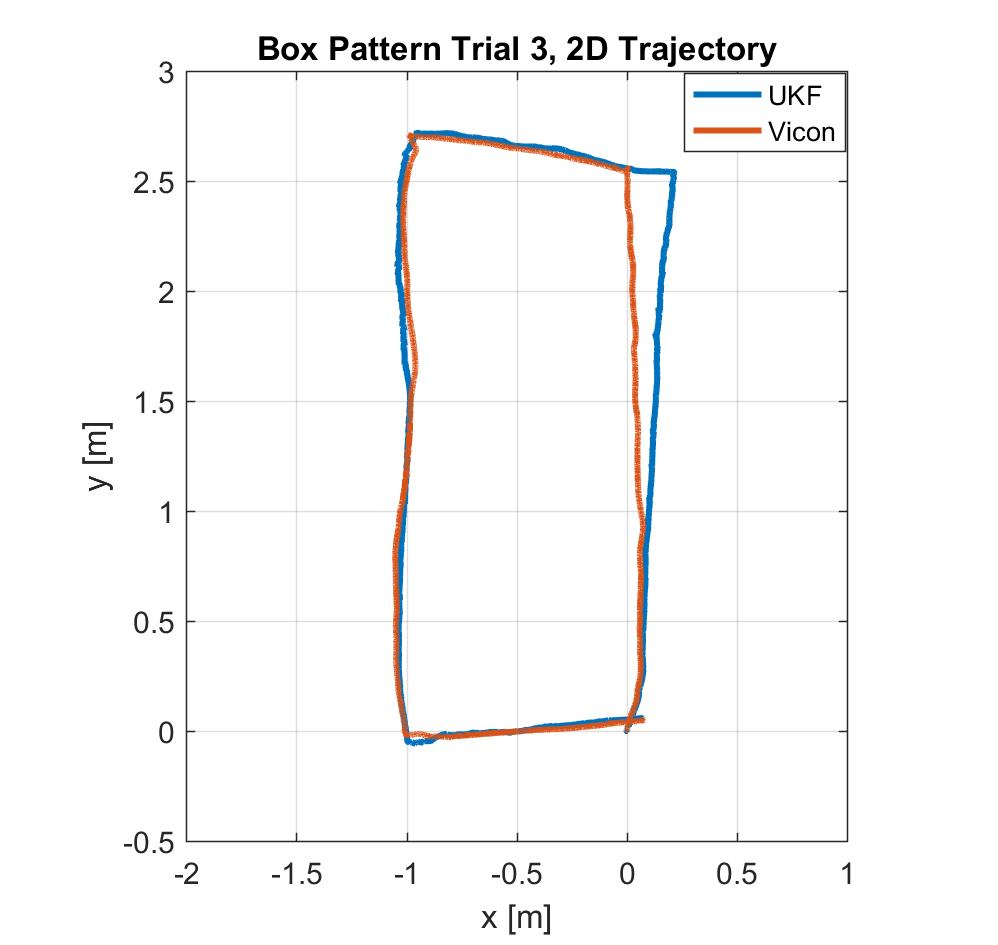
\includegraphics[height=0.6\textwidth]{box3_2d}
  \caption[Box Pattern Trial 3 2D Trajectory]{Box Pattern Trial 3 2D Trajectory.}
  \label{fig:box3_2d}
\end{figure}
\begin{figure}[p]
  \centering
    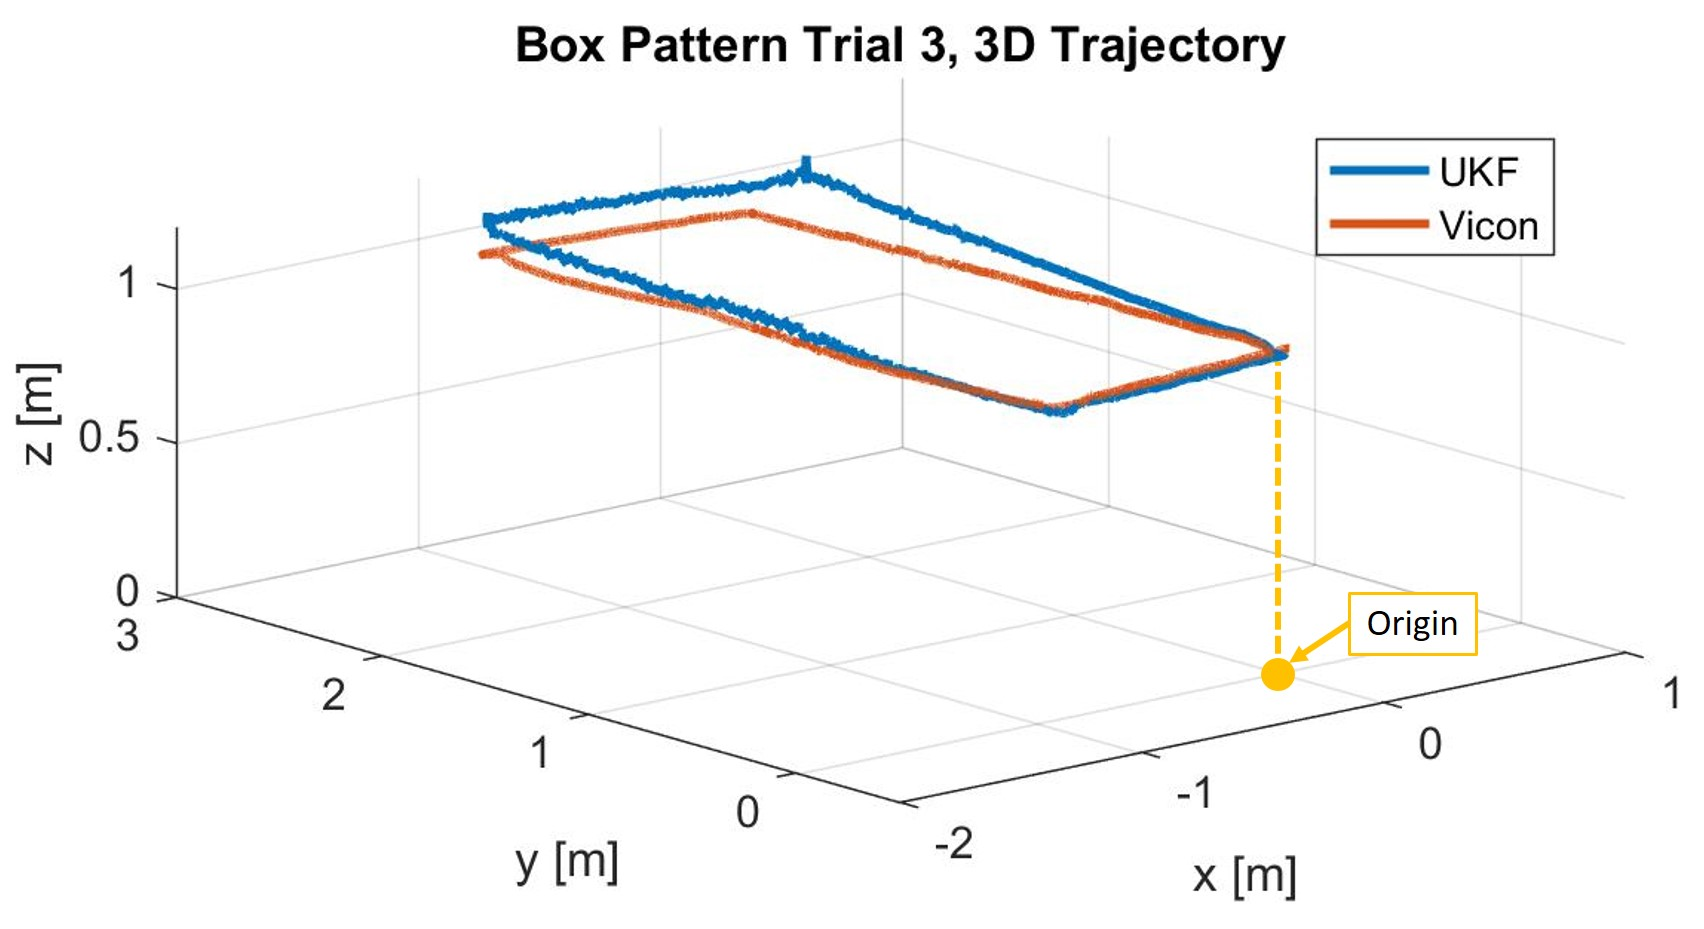
\includegraphics[height=0.7\textwidth]{box3_3d}
  \caption[Box Pattern Trial 3 3D Trajectory]{Box Pattern Trial 3 3D Trajectory.}
  \label{fig:box3_3d}
\end{figure}
\clearpage

% Box 4
\begin{figure}[p]
  \centering
    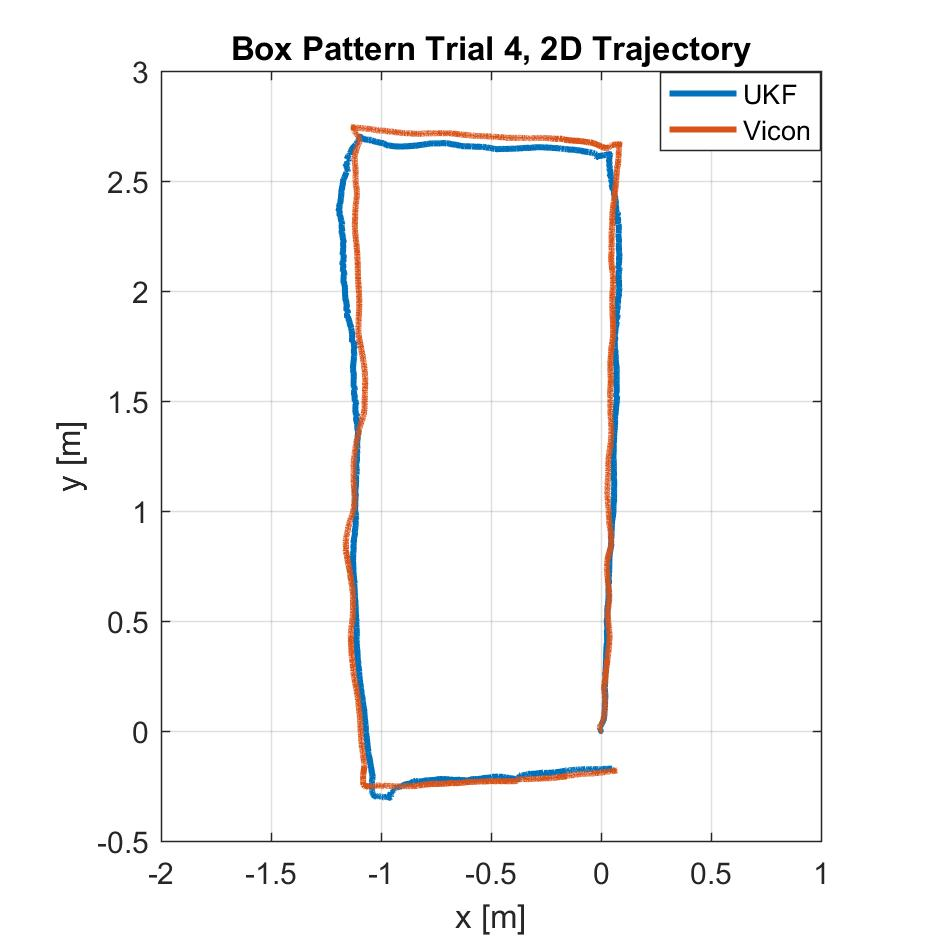
\includegraphics[height=0.6\textwidth]{box4_2d}
  \caption[Box Pattern Trial 4 2D Trajectory]{Box Pattern Trial 4 2D Trajectory.}
  \label{fig:box4_2d}
\end{figure}
\begin{figure}[p]
  \centering
    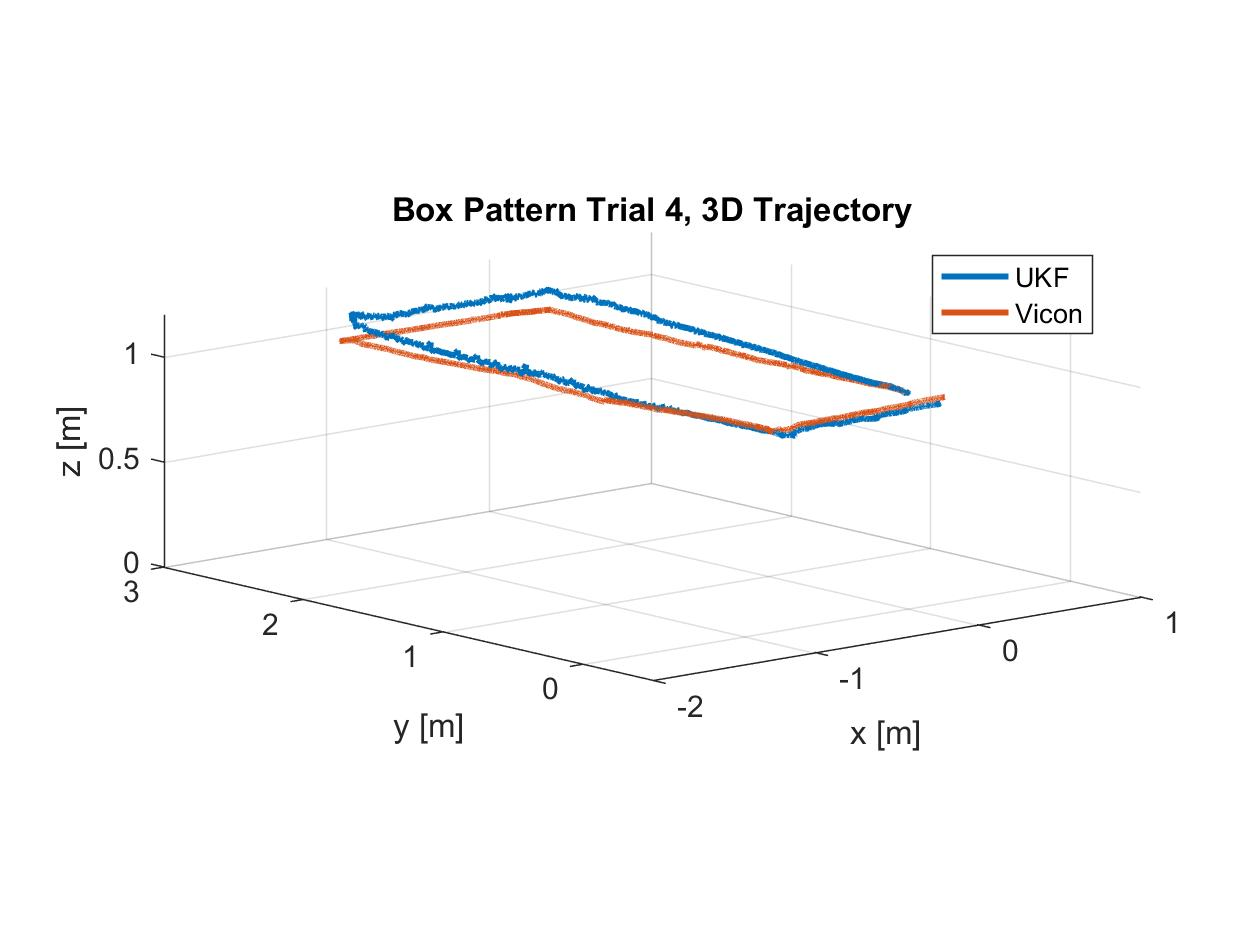
\includegraphics[height=0.7\textwidth]{box4_3d}
  \caption[Box Pattern Trial 4 3D Trajectory]{Box Pattern Trial 4 3D Trajectory.}
  \label{fig:box4_3d}
\end{figure}
\clearpage

% Box 5
\begin{figure}[p]
  \centering
    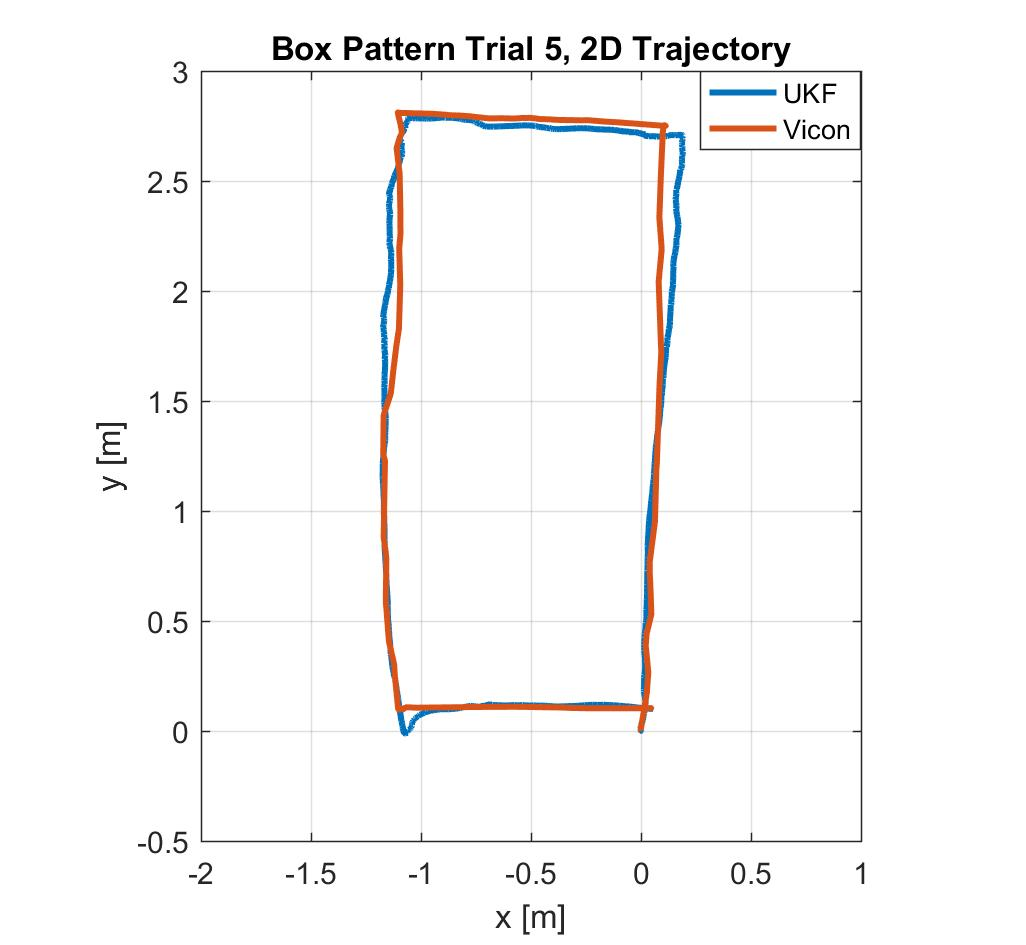
\includegraphics[height=0.6\textwidth]{box5_2d}
  \caption[Box Pattern Trial 5 2D Trajectory]{Box Pattern Trial 5 2D Trajectory.}
  \label{fig:box5_2d}
\end{figure}
\begin{figure}[p]
  \centering
    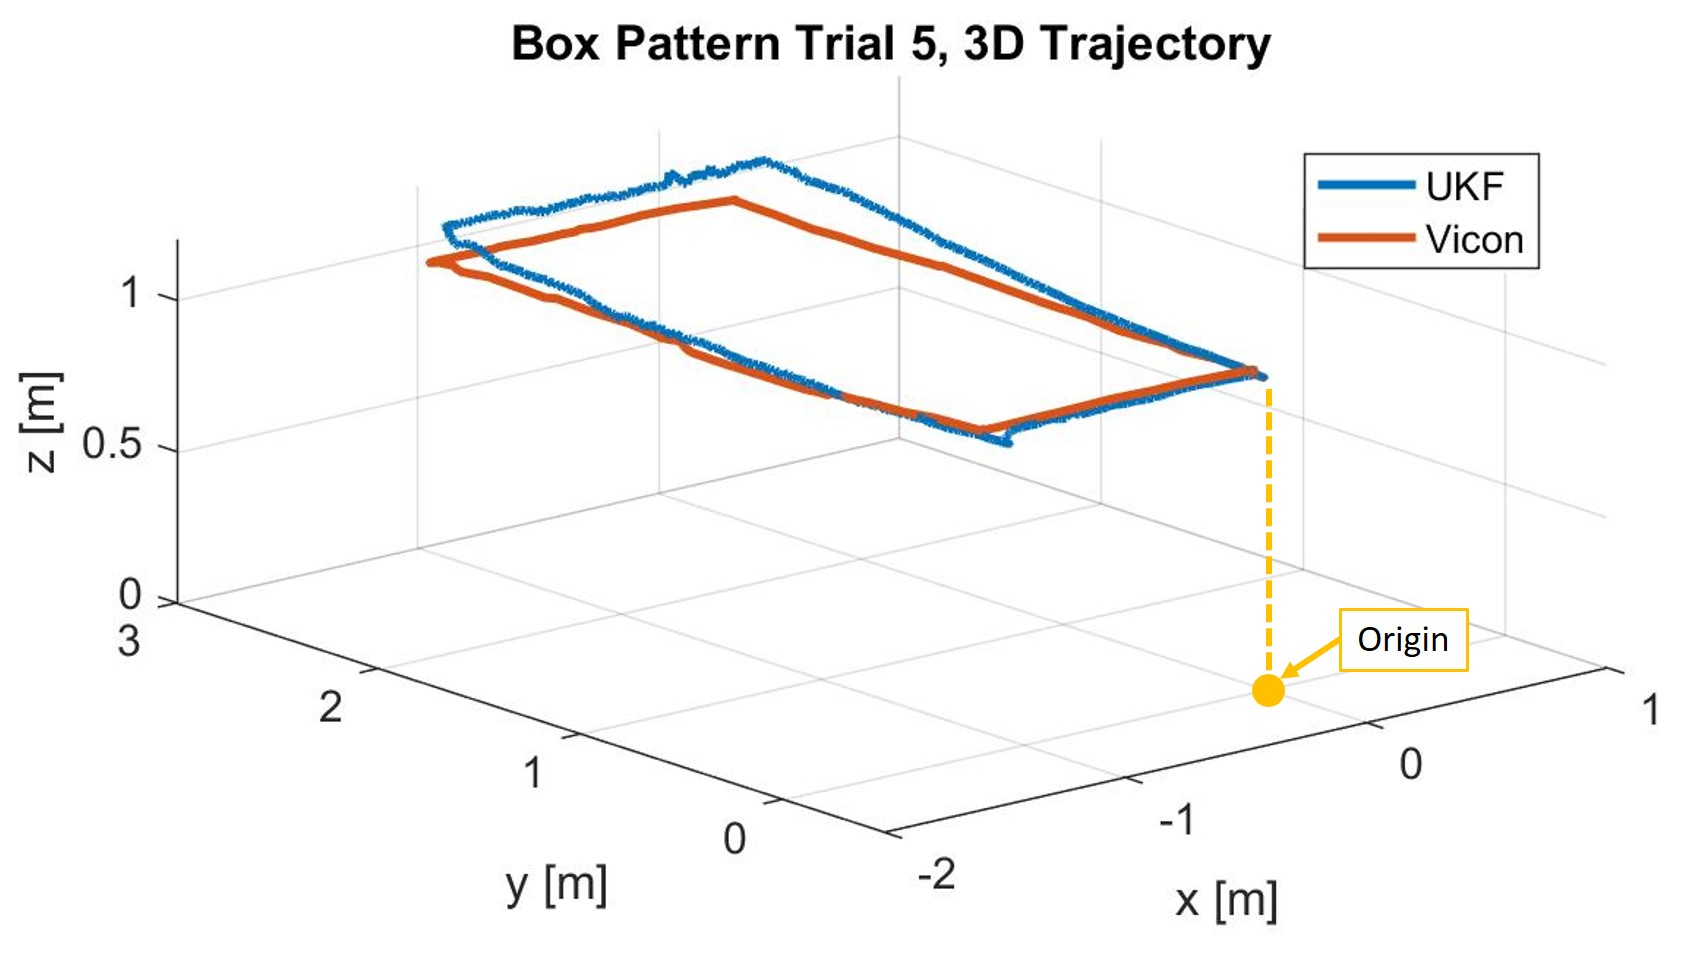
\includegraphics[height=0.7\textwidth]{box5_3d}
  \caption[Box Pattern Trial 5 3D Trajectory]{Box Pattern Trial 5 3D Trajectory.}
  \label{fig:box5_3d}
\end{figure}
\clearpage

\section{Error Analysis}

To determine the effectiveness of the UKF framework in estimating the position of a vehicle, we develop a number of statistical metrics to characterize the varieties and magnitudes of error in the filter's output. In this section, we perform statistical analyses on the data streams collected during the box pattern trials. The positional error in the long walk trials is effectively unbounded. Because of the bowl-shaped lens distortion defect mentioned previously, moving the vehicle in long translations produces ever-increasing altitudinal error and distorts lateral sensitivity. As a result, we examine only the box pattern trials to characterize the system's error in a scenario where the combination of sensors being used would be a more reasonable choice.

Positional errors in the UKF output were computed after each trial per the following relationships:
%
\begin{align}
\varepsilon_{x} &= x_{\text{Vicon}} - x_{\text{UKF}} \\
\varepsilon_{y} &= y_{\text{Vicon}} - y_{\text{UKF}} \\
\varepsilon_{z} &= z_{\text{Vicon}} - z_{\text{UKF}}
\end{align}
%
These positional errors were computed over the length of each coordinate time history, creating an error history for each trial. The mean coordinate errors and their variances were then computed from these error histories to characterize the Gaussian noise distribution in each data set. The terms $\mu_{x}$, $\mu_{y}$, and $\mu_{z}$ encode the mean error in $x$, $y$, and $z$, respectively. The associated variances of these errors are represented by $\sigma_{x}^{2}$, $\sigma_{y}^{2}$, and $\sigma_{z}^{2}$. These statistics are presented in Table~\ref{tab:means_and_vars}.

\begin{table}[h]\centering
\caption[Coordinate Error]{Coordinate error mean and variance values by trial.}
\begin{tabular}[c]{crr|rr|rr}
\toprule
Trial & $\mu_{x}$ [m] & $\sigma_{x}^{2}$ [m$^{2}$] & $\mu_{y}$ [m] & $\sigma_{y}^{2}$ [m$^{2}$] & $\mu_{z}$ [m] & $\sigma_{z}^{2}$ [m$^{2}$] \\
\hline
1 & $-$0.0048 & 9.4976e$-$04 & 0.0126 & 2.6861e$-$04 & $-$0.0247 & 0.0015 \\
2 & $-$0.0084 & 0.0013 & 0.0079 & 1.9425e$-$04 & $-$0.0583 & 0.0030 \\
3 & $-$0.0341 & 0.0043 & 0.0033 & 1.9481e$-$04 & $-$0.0333 & 0.0028 \\
4 & $-$3.9788e$-$04 & 7.5902e$-$04 & 0.0199 & 8.0152e$-$04 & $-$0.0219 & 0.0033 \\
5 & $-$0.0170 & 0.0019 & 0.0279 & 0.0036 & $-$0.0372 & 0.0034 \\
\hline
\textbf{Grand Mean} & $-$0.0129 &  & 0.0143 &  & $-$0.0351 & \\
\bottomrule
\end{tabular}
\label{tab:means_and_vars}
\end{table}

The positional errors were composed into a positional error vector $\bm{\varepsilon}$ describing the offset between ground truth and the estimated trajectory at a given point in time:
%
\begin{equation}
\bm{\varepsilon} = \left\lbrace \varepsilon_{x},\ \varepsilon_{y},\ \varepsilon_{z} \right\rbrace ^{T}
\end{equation}
%
The norm of this error vector is the total Euclidean offset $\| \bm{\varepsilon} \|$:
%
\begin{equation}
\| \bm{\varepsilon} \| = \sqrt{\varepsilon_{x}^{2} + \varepsilon_{y}^{2} + \varepsilon_{z}^{2}} 
\end{equation}
%
The total Euclidean offset encodes the straight-line distance between the ground truth position and the estimated position, providing a measure of total positional error at each point in time. The total Euclidean offset was computed over the entire error history in order to characterize the evolution of the error over time. This magnitudinal error history was then analyzed for each experimental trial in order to determine the mean total error and maximum total error ($\| \bm{\varepsilon} \|_{\text{max.}}$). These statistics are presented in Table~\ref{tab:total_err}.

\begin{table}[h]\centering
\caption[Mean and Maximum Total Error]{Mean and maximum total error by trial.}
\begin{tabular}[c]{crr}
\toprule
Trial & Mean $\| \bm{\varepsilon} \|$ [m] & $\| \bm{\varepsilon} \|_{\text{max.}}$ [m] \\
\hline
1 & 0.0460 & 0.1145 \\
2 & 0.0691 & 0.1999 \\
3 & 0.0695 & 0.2596 \\
4 & 0.0636 & 0.1508 \\
5 & 0.0856 & 0.2497 \\
\hline
\textbf{Grand Mean} & 0.0668 \\
\hline
\textbf{Maximum Error} && 0.2596 \\
\bottomrule
\end{tabular}
\label{tab:total_err}
\end{table}

From Table~\ref{tab:means_and_vars}, we can see that the mean coordinate errors are (1) small in magnitude, being less than 4~cm in any direction, and (2) close to zero, supporting our intuition of a zero-mean Gaussian distribution. The variance values are also small in magnitude, being on the order of $10^{-3}$~m$^{2}$ or less in all cases. This indicates a tight distribution of error about the mean, implying that large erroneous spikes were rare during testing. Table~\ref{tab:total_err} shows that the system ran with a mean total error of 0.0668~m and a maximum error of 0.2596~m. This indicates that the system was able to estimate the vehicle's position consistently with sub-meter accuracy over the length of each trial. The maximum error, though large, still falls well within the 4.9-m radius generally realizable with current smartphone GPS receivers (\cite{GpsGov}), indicating that the system could prove to be a reasonable choice for outdoor navigation or for indoor navigation in open areas where centimeter-level accuracy would not be required.